%
% $RCSfile: practical_proof.tex,v $
%
% Copyright (c) 2005-2006. Christian Heller. All rights reserved.
%
% Permission is granted to copy, distribute and/or modify this document
% under the terms of the GNU Free Documentation License, Version 1.1 or
% any later version published by the Free Software Foundation; with no
% Invariant Sections, with no Front-Cover Texts and with no Back-Cover
% Texts. A copy of the license is included in the section entitled
% "GNU Free Documentation License".
%
% http://www.cybop.net
% - Cybernetics Oriented Programming -
%
% http://www.resmedicinae.org
% - Information in Medicine -
%
% Version: $Revision: 1.1 $ $Date: 2006-01-03 08:21:45 $ $Author: christian $
% Authors: Christian Heller <christian.heller@tuxtax.de>
%

\section{Practical Proof}
\label{practical_proof_heading}

The proof of operatability for the new concepts is given by the
\emph{Cybernetics Oriented Language} (CYBOL), defined according to the
principles of abstraction worked out before, and by the
\emph{Cybernetics Oriented Interpreter} (CYBOI), a knowledge processing system.
In addition, a prototype application called \emph{Res Medicinae}
\cite{resmedicinae} was implemented in CYBOL, but will -- due to the limited
space -- not be explained further here.

%
% $RCSfile: document_type_definition.tex,v $
%
% Copyright (c) 2002-2007. Christian Heller. All rights reserved.
%
% Permission is granted to copy, distribute and/or modify this document
% under the terms of the GNU Free Documentation License, Version 1.1 or
% any later version published by the Free Software Foundation; with no
% Invariant Sections, with no Front-Cover Texts and with no Back-Cover
% Texts. A copy of the license is included in the section entitled
% "GNU Free Documentation License".
%
% http://www.cybop.net
% - Cybernetics Oriented Programming -
%
% Version: $Revision: 1.2 $ $Date: 2007-08-01 13:59:00 $ $Author: christian $
% Authors: Christian Heller <christian.heller@tuxtax.de>
%

\subsection{Document Type Definition}
\label{document_type_definition_heading}
\index{Document Type Definition}
\index{DTD}
\index{Extensible Markup Language}
\index{XML}
\index{Markup Tag}
\index{model Tag}
\index{part Tag}
\index{property Tag}
\index{constraint Tag}
\index{name Attribute}
\index{channel Attribute}
\index{abstraction Attribute}
\index{model Attribute}

A DTD represents the type definition of an XML document. It consists of a set
of \emph{Markup Tags} and their \emph{Interpretation} \cite{foldoc}. DTDs can
be declared inline, within a document, or as an external reference
\cite{w3schools}. Figure \ref{dtd_figure} shows the DTD of the CYBOL language.

\begin{figure}[ht]
    \bigskip
    \begin{scriptsize}
        \begin{verbatim}
<!ELEMENT model (part*)>
<!ELEMENT part (property*)>
<!ELEMENT property (constraint*)>
<!ELEMENT constraint EMPTY>

<!ATTLIST part
    name CDATA #REQUIRED
    channel CDATA #REQUIRED
    abstraction CDATA #REQUIRED
    model CDATA #REQUIRED>
<!ATTLIST property
    name CDATA #REQUIRED
    channel CDATA #REQUIRED
    abstraction CDATA #REQUIRED
    model CDATA #REQUIRED>
<!ATTLIST constraint
    name CDATA #REQUIRED
    channel CDATA #REQUIRED
    abstraction CDATA #REQUIRED
    model CDATA #REQUIRED>
        \end{verbatim}
    \end{scriptsize}
    \caption{Recommended CYBOL DTD}
    \label{dtd_figure}
\end{figure}

Following the pure hierarchical structure of CYBOL, it would actually suffice
to use a DTD as simple as the one shown in figure \ref{simpledtd_figure}. Since
the three elements \emph{part}, \emph{property} and \emph{constraint} (compare
figure \ref{dtd_figure}) have the same list of required attributes, they could
be summarised under the name \emph{part}, for example. Because the structure of
a CYBOL model is non-ambiguous, the meaning of its elements can be guessed from
their position within the model.

\begin{figure}[ht]
    \bigskip
    \begin{scriptsize}
        \begin{verbatim}
<!ELEMENT part (part*)>

<!ATTLIST part
    name CDATA #REQUIRED
    channel CDATA #REQUIRED
    abstraction CDATA #REQUIRED
    model CDATA #REQUIRED>
        \end{verbatim}
    \end{scriptsize}
    \caption{Simplified CYBOL DTD}
    \label{simpledtd_figure}
\end{figure}

\clearpage

For the purpose of expressing knowledge in accordance with the schema suggested
by CYBOP \cite{cybop}, a CYBOL knowledge template (file) does not need to have
a root element. The file name clearly identifies it. For reasons of XML
conformity, however, an extra root element called \emph{model} was defined
(figure \ref{dtd_figure}). And for reasons of better readability and
programmability, the three kinds of embedded elements were given distinct names.

%
% $RCSfile: hello_world.tex,v $
%
% Copyright (c) 2005-2006. Christian Heller. All rights reserved.
%
% Permission is granted to copy, distribute and/or modify this document
% under the terms of the GNU Free Documentation License, Version 1.1 or
% any later version published by the Free Software Foundation; with no
% Invariant Sections, with no Front-Cover Texts and with no Back-Cover
% Texts. A copy of the license is included in the section entitled
% "GNU Free Documentation License".
%
% http://www.cybop.net
% - Cybernetics Oriented Programming -
%
% http://www.resmedicinae.org
% - Information in Medicine -
%
% Version: $Revision: 1.1 $ $Date: 2006-01-03 08:21:45 $ $Author: christian $
% Authors: Christian Heller <christian.heller@tuxtax.de>
%

\subsection{Hello World}
\label{hello_world_heading}

The well-known \emph{Hello, World!} program printing just two words shall be
given as minimal example application. It consists of only two operations:
\emph{send} and \emph{exit}. The string message to be displayed on screen is
handed over as \emph{property} to the \emph{send} operation, before the
\emph{exit} shuts down the system:

\begin{scriptsize}
    \begin{verbatim}
<model>
    <part name="send_model_to_output"
        channel="inline"
        abstraction="operation"
        model="send">
        <property name="language"
            channel="inline"
            abstraction="string"
            model="tui"/>
        <property name="receiver"
            channel="inline"
            abstraction="string"
            model="user"/>
        <property name="message"
            channel="inline"
            abstraction="string"
            model="Hello, World!"/>
    </part>
    <part name="exit_application"
        channel="inline"
        abstraction="operation"
        model="exit"/>
</model>
    \end{verbatim}
\end{scriptsize}

%
% $RCSfile: container_mapping.tex,v $
%
% Copyright (c) 2002-2007. Christian Heller. All rights reserved.
%
% Permission is granted to copy, distribute and/or modify this document
% under the terms of the GNU Free Documentation License, Version 1.1 or
% any later version published by the Free Software Foundation; with no
% Invariant Sections, with no Front-Cover Texts and with no Back-Cover
% Texts. A copy of the license is included in the section entitled
% "GNU Free Documentation License".
%
% http://www.cybop.net
% - Cybernetics Oriented Programming -
%
% Version: $Revision: 1.1 $ $Date: 2007-08-01 13:59:00 $ $Author: christian $
% Authors: Christian Heller <christian.heller@tuxtax.de>
%

\section{Container Mapping}
\label{container_mapping_heading}
\index{Containers in CYBOL}
\index{Mapping Containers to CYBOL}

State-of-the-art programming languages like Java offer a number of different
container types (figure \ref{container_figure}).

\begin{figure}[ht]
    \begin{center}
        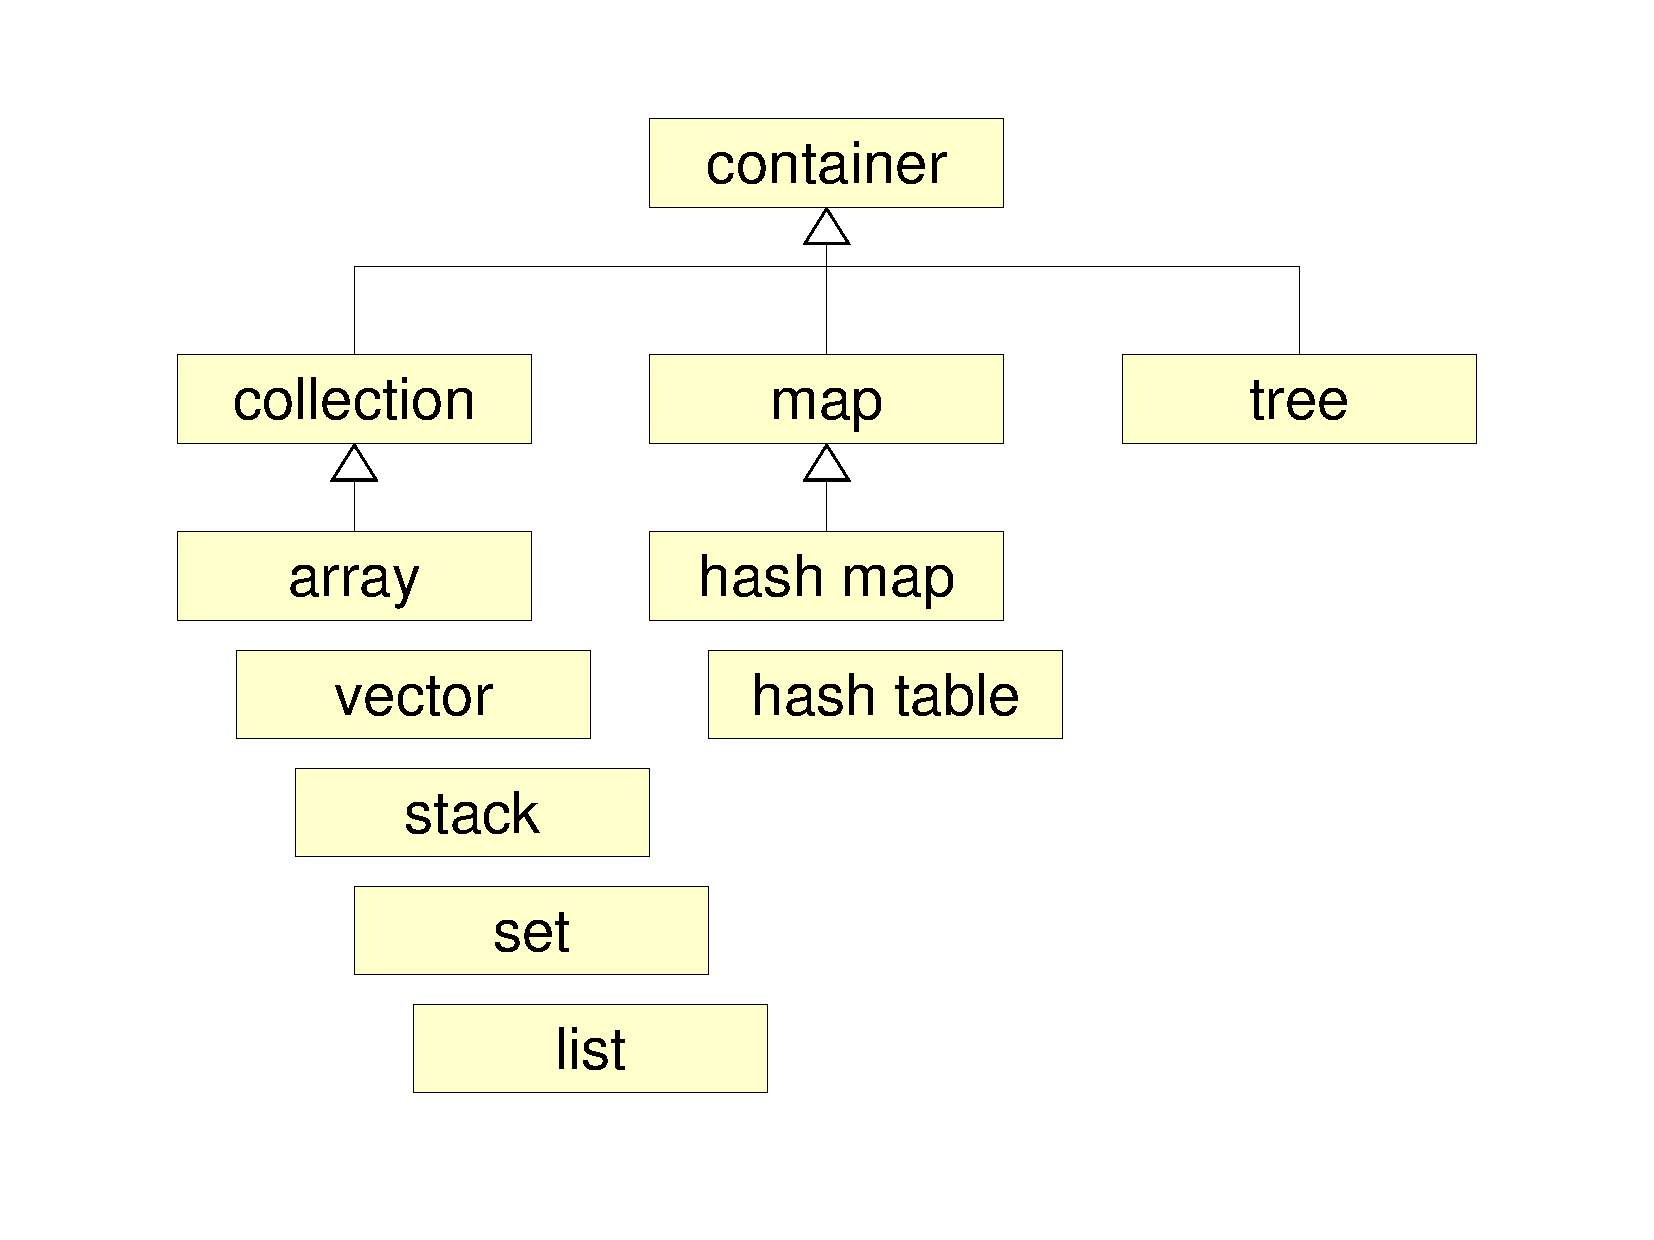
\includegraphics[scale=0.3,angle=-90]{graphics/container.pdf}
        \caption{Classical Container Types in Java}
        \label{container_figure}
    \end{center}
\end{figure}

\begin{table}[ht]
    \begin{center}
        \begin{footnotesize}
        \begin{tabular}{| p{35mm} | p{70mm} |}
            \hline
            \textbf{Classical Container Type} & \textbf{Realisation in CYBOL Knowledge Template}\\
            \hline
            Tree & Hierarchical \emph{whole}-\emph{part} structure\\
            \hline
            Table & Like a Tree, as hierarchy consisting of rows which consist of columns\\
            \hline
            Map & Parts have a \emph{name} (key) and a \emph{model} (value)\\
            \hline
            List & Parts may have a \emph{position} property\\
            \hline
            Vector & A \emph{model} attribute may hold comma-separated values;
                an extra template holds a dynamically changeable number of parts\\
            \hline
            Array & Like a Vector; characters are interpreted as \emph{string}\\
            \hline
        \end{tabular}
        \end{footnotesize}
        \caption{Mapping Classical Containers to CYBOL}
        \label{mapping_table}
    \end{center}
\end{table}

CYBOI owns a \emph{Knowledge Schema} which represents each item as
\emph{Hierarchy} by default, the result being that different types of
containers are \emph{not} needed any longer, that is are unified. Table
\ref{mapping_table} shows how the different kinds of container behaviour are
implemented in CYBOL. As can be seen, CYBOL is able to represent many container
types.

%
% $RCSfile: knowledge_handling_system.tex,v $
%
% Copyright (c) 2005-2006. Christian Heller. All rights reserved.
%
% Permission is granted to copy, distribute and/or modify this document
% under the terms of the GNU Free Documentation License, Version 1.1 or
% any later version published by the Free Software Foundation; with no
% Invariant Sections, with no Front-Cover Texts and with no Back-Cover
% Texts. A copy of the license is included in the section entitled
% "GNU Free Documentation License".
%
% http://www.cybop.net
% - Cybernetics Oriented Programming -
%
% http://www.resmedicinae.org
% - Information in Medicine -
%
% Version: $Revision: 1.1 $ $Date: 2006-01-03 08:21:45 $ $Author: christian $
% Authors: Christian Heller <christian.heller@tuxtax.de>
%

\subsection{Knowledge-handling System}
\label{knowledge_handling_system_heading}

The pure existence of proper knowledge does not suffice to create an improved
kind of software system, within a slimmer software development process. The
system needs to know how to \emph{handle} knowledge, at runtime. The criticism
is twofold, since traditionally:

\begin{enumerate}
    \item Operating systems don't have sufficient knowledge handling capabilities
    \item Applications contain too much low-level system control functionality
\end{enumerate}

This is changed when using CYBOI. As active interpreter encapsulating
system-level functionality, it handles knowledge provided in form of passive
CYBOL templates. In CYBOP systems, all compound knowledge models have the same
type structure (schema). Since they do not differ, they can be manipulated in
the same manner.

\begin{figure}[ht]
    \begin{center}
        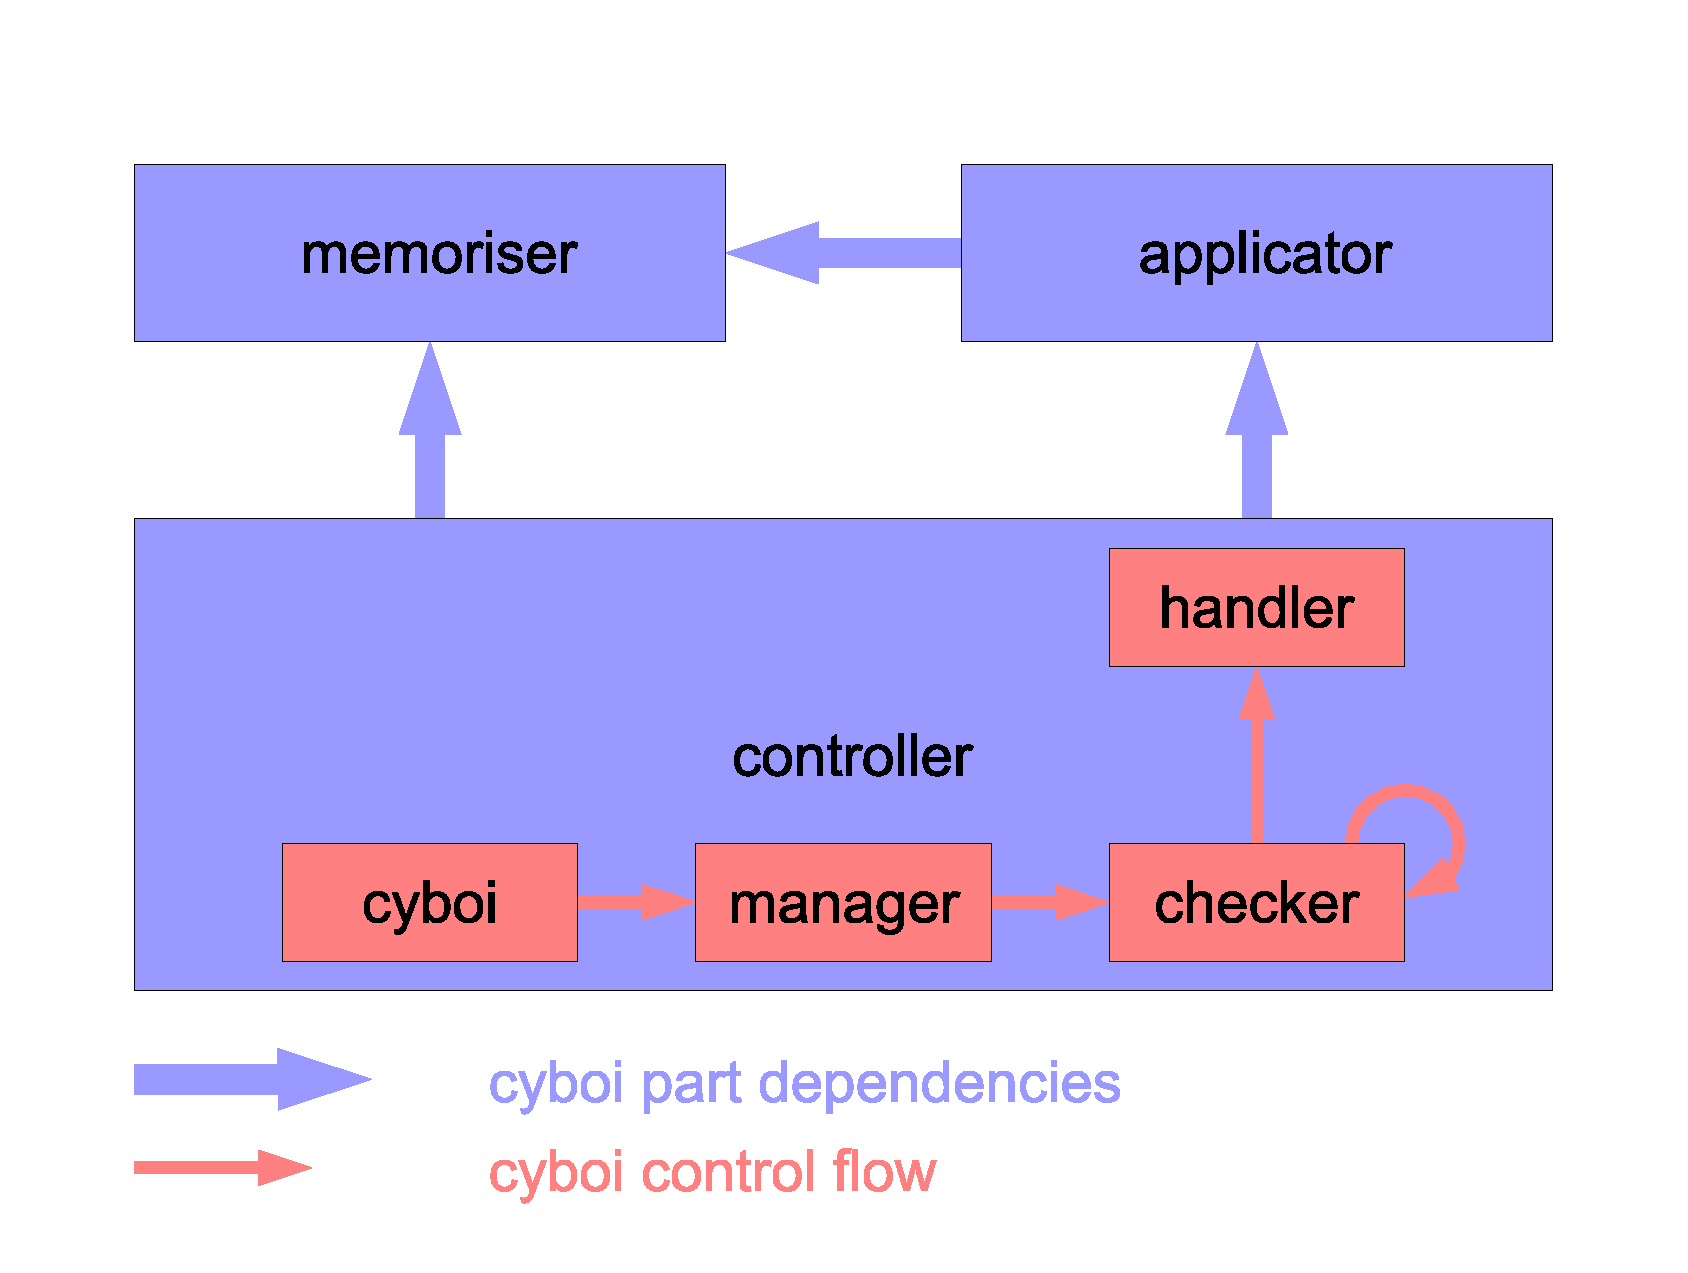
\includegraphics[scale=0.2]{vector/dependencies.eps}
        \caption{CYBOI Architecture}
        \label{cyboi_figure}
    \end{center}
\end{figure}

Figure \ref{cyboi_figure} shows three main parts of CYBOI: The
\emph{Controller} manages system startup, shutdown and the handling of signals
during its runtime; the system uses just one central signal checking loop. The
\emph{Memoriser} provides memory structures (to store knowledge) and procedures
to access these. Logic knowledge is processed in the \emph{Applicator}.
Parallels to the \emph{von Neumann} architecture \cite{selflinux} are intended.

